\begin{surferPage}[Sestica di Barth]{La Sestica di Barth}
    Questa superficie di grado $6$ (sestica) fu costruita da Wolf Barth nel 1996.
    
    La Sestica di Barth ha in tutto $65$ singolarit\`a.
%    (wenn man die $15$ im Bild nicht sichtbaren, ``unendlich fernen'', mitz�hlt)%
   Questo \`e il massimo numero possibile di singolarit\`a su una sestica, come mostrato da Jaffe e Ruberman poco dopo la costruzione di Barth --- quindi il record mondiale di Barth \`e imbattibile!

La costruzione di Barth fu una grande sorpresa perch\'e per lungo tempo si pens\`o che le superfici di grado $6$ potessero avere al massimo $64$ singolarit\`a.

Una straordinaria caratteristica di questa costruzione \`e la sua simmetria icosaedrale; la figura mostra un icosaedro e i suoi piani di simmetria:
  \begin{center}
      \vspace*{-0.1cm}
      \begin{tabular}{@{}c@{\ \ }c@{\,}c@{}}
        \begin{tabular}{@{}c}
          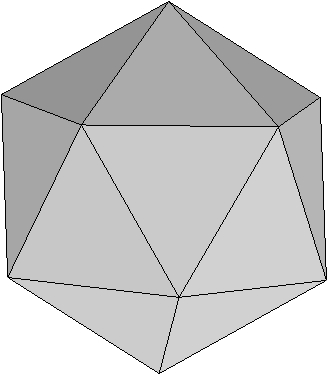
\includegraphics[width=1.4cm]{./../../common/images/icosah}
        \end{tabular}
        &
        \begin{tabular}{@{}c}
          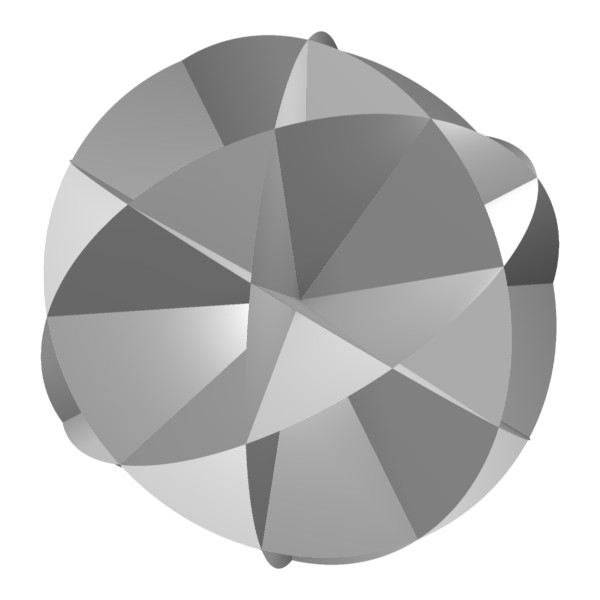
\includegraphics[width=1.4cm]{./../../common/images/barth_sextic_planes}
        \end{tabular}
        &
        \begin{tabular}{c@{}}
          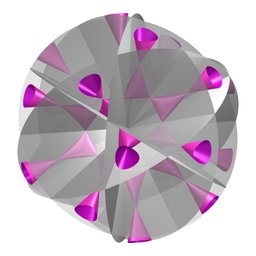
\includegraphics[width=1.4cm]{./../../common/images/barth_sextic_and_planes}
        \end{tabular}
      \end{tabular}
    \end{center}
    \vspace*{-0.1cm}

    La Sestica di Barth soddisfa l'equazione $P_6 - \alpha K^2=0,$ dove $P_6$ indica i sei piani di simmetria, $K=x^2+y^2+z^2-1$ \`e la sfera unitaria e 
    $\alpha=\frac{1}{4}(2+\sqrt{5})$.
\end{surferPage}
